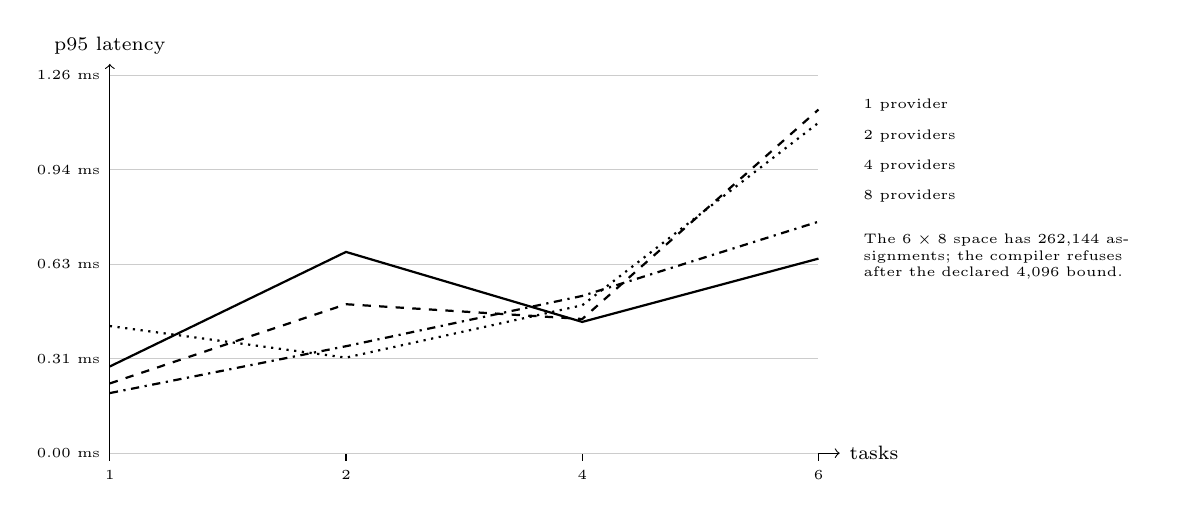
\begin{tikzpicture}[x=9cm,y=4.8cm]
\draw[->] (0,0)--(1.03,0) node[right]{\scriptsize tasks};
\draw[->] (0,0)--(0,1.03) node[above]{\scriptsize p95 latency};
\draw (0.0000,0)--(0.0000,-0.02) node[below]{\tiny 1};
\draw (0.3333,0)--(0.3333,-0.02) node[below]{\tiny 2};
\draw (0.6667,0)--(0.6667,-0.02) node[below]{\tiny 4};
\draw (1.0000,0)--(1.0000,-0.02) node[below]{\tiny 6};
\draw[black!20] (0,0.00)--(1,0.00);\node[left,font=\tiny] at (0,0.00) {0.00 ms};
\draw[black!20] (0,0.25)--(1,0.25);\node[left,font=\tiny] at (0,0.25) {0.31 ms};
\draw[black!20] (0,0.50)--(1,0.50);\node[left,font=\tiny] at (0,0.50) {0.63 ms};
\draw[black!20] (0,0.75)--(1,0.75);\node[left,font=\tiny] at (0,0.75) {0.94 ms};
\draw[black!20] (0,1.00)--(1,1.00);\node[left,font=\tiny] at (0,1.00) {1.26 ms};
\draw[thick,solid] (0.0000,0.2294) -- (0.3333,0.5325) -- (0.6667,0.3473) -- (1.0000,0.5148);
\node[anchor=west,font=\tiny] at (1.05,0.92) {1 provider};
\draw[thick,dashed] (0.0000,0.1846) -- (0.3333,0.3941) -- (0.6667,0.3550) -- (1.0000,0.9091);
\node[anchor=west,font=\tiny] at (1.05,0.84) {2 providers};
\draw[thick,dotted] (0.0000,0.3364) -- (0.3333,0.2528) -- (0.6667,0.3914) -- (1.0000,0.8742);
\node[anchor=west,font=\tiny] at (1.05,0.76) {4 providers};
\draw[thick,dash dot] (0.0000,0.1590) -- (0.3333,0.2830) -- (0.6667,0.4161) -- (1.0000,0.6126);
\node[anchor=west,font=\tiny] at (1.05,0.68) {8 providers};
\node[anchor=west,font=\tiny,text width=36mm] at (1.05,0.52) {The $6\times8$ space has 262,144 assignments; the compiler refuses after the declared 4,096 bound.};
\end{tikzpicture}
